\taskpic{ Прямоугольный сосуд с водой стоит на двух опорах,
  разнесенных на расстояние $L$ друг от друга. Над сосудом на
  перекладине подвешен на нити кусок свинца массой $M$ на расстоянии
  $l$ от центра сосуда. Силы реакции опор равны при этом $N_1$ и
  $N_2$. Нить удлиняют так, что свинец погружается в воду. Какими
  станут после этого силы реакции опор? Плотность свинца в $n$ раз
  больше плотности воды.  }{
  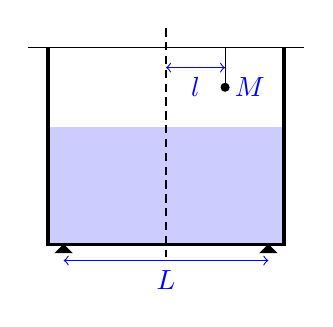
\begin{tikzpicture}
    \fill[fill=blue!20] (0.5,0.5) rectangle (3.5,2);
    \draw[very thick] (0.5,3) -- (0.5,0.5) -- (3.5,0.5) -- (3.5,3);
    \draw (0.25,3) -- (3.75,3);
    \draw (2.75,3) -- ++(0,-0.5);
    \filldraw (2.75,2.5) circle (0.05cm) node [blue,right] {$M$};
    \draw[densely dashed] (2,3.25) -- (2,0.35);
    \draw[blue,<->] (2,2.75) -- (2.75,2.75) node[midway,below] {$l$};
    \filldraw (0.7,0.5) -- ++(-0.1,-0.1) -- ++(0.2,0) -- cycle;
    \filldraw (3.3,0.5) -- ++(-0.1,-0.1) -- ++(0.2,0) -- cycle;
    \draw[blue,<->] (0.7,0.3) -- (3.3,0.3) node[below,midway] {$L$};
  \end{tikzpicture}
}
